\documentclass[]{article}
\usepackage{huy}
\pagestyle{empty}
\usepackage[margin=2cm]{geometry}
\begin{document}
\intro{DATABASE}{Enhanced ER modeling}
\section{Specialization/Generalization}
The concept of Specialization/Generalization is associated with special types of entities known as \emph{superclasses} and \emph{subclasses}, and the process of \emph{attribute inheritance}.
\begin{description}
\item[Superclasses] An entity type that includes one or more distinct sub-groupings of its occurrences, which must be represented in a data model.
\item[Subclasses] A distinct sub-grouping of occurrences of an entity type, which must be represented in a data model.
\end{description}
Each member of a subclass is also a member of the superclass. In other words, the entity in the subclass is the same entity in the superclass, but has a distinct role. The relationship between  a superclass and a subclass is one-to-one and is called a superclass/subclass relationship. However, not every member of a superclass is necessarily a member of a subclass; for example, members of staff without a distinct job such as a Manager or a member of Sales Personnel.\par 
We can use superclasses and subclasses to avoid describing different types of staff with possibly different attributes within a single entity. For example, Sales Personnel may have a special attributes such as salesArea and carAllowance. If all staff attributes and those specific to particular jobs (such as salesArea and carAllowance of Sales Personnel) are described by a single entity Staff entity, this may result in a lot of nulls for the job-specific attributes.\par 
A subclass is an entity in its own right and so it may also have one or more subclasses. An entity and its subclasses and their subclasses, and so on, is called a \emph{type hierarchy}. Type hierarchies are known by a varieties of names including \emph{specialization hierarchy} (e.g. Manager is a specialization of Staff), \emph{generalization hierarchy} (e.g. Staff is a generalization of Manager), and \emph{IS-A hierarchy} (e.g. Manager IS-A (member of) Staff).
\begin{description}
\item[Specialization]The process of maximizing the differences between members of an entity by identifying their distinguish characteristics.
\item[Generalization]The process of minimizing the differences between members of an entity by identifying their common characteristics.
\end{description}
\section{Aggregation}
Aggregation represents a ``has a'' or ``is a part of'' relationship between entity types, where one represents the ``whole'' and the other the ``part''. This relationship represents an association between two entity types that are at the same level. Composition is a specific form of aggregation that represents an association between entities, where there is a strong ownership and coincidental lifetime between the ``whole'' and the ``part''. An object may be part of only one composite at a time. In a composite, when the ``whole'' is deleted, all the ``parts'' of it are deleted as well.
\section{UML diagrammatic notation}
UML has a special notation for representing Specialization/Generalization and aggregation. As for Specialization/Generalization, the subclasses are attached by lines to a triangle that point towards the superclass. When it comes to aggregation, UML use an open diamond shape at one end of the relationship line, next to the entity that represents the ``whole''. A filled-in diamond shape replaces open diamond when representing composition.\par 
Let's create an ER model for the following description:
School of Engineering has many departments. There are students in the
School Of Engineering. Hopefully, each student attends to one or more
courses. Each department supplies one or more courses. There are one or
more instructors (teachers) in each department.
\begin{figure}[hbtp]
\caption{UML class notation}
\centering
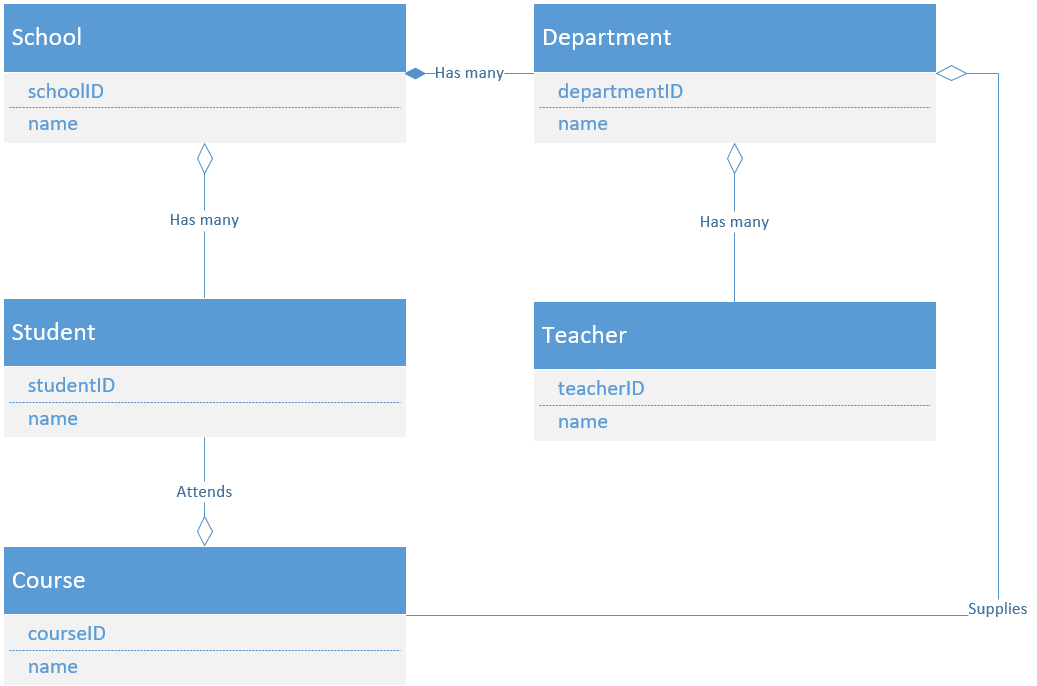
\includegraphics[width=\textwidth]{Capture.PNG}
\end{figure}

\end{document}